\section{Introduction}

\subsection{The Structure-Function Problem in Neuroscience}
It is considered paradigmatic in neuroscience that the brain's structure
at various spatial scales is critical for determining its function. In
particular, the relationship between the brain's \emph{structural
wiring} and the \emph{functional} patterns of neural activity is of
fundamental interest in computational neuroscience. Brain structure and
function at the scale of macroscopic networks, i.e. amongst identifiable
grey matter (GM) regions and their long-range connections through white
matter (WM) fiber bundles, can be adequately measured using current
non-invasive measurement techniques. Fiber architecture can be measured
from diffusion tensor imaging (DTI) followed by tractography algorithms
\cite{hagmann_mapping_2008,iturria-medina_anatomical_2013}. Similarly, brain function manifested in neural
oscillations can be measured non-invasively using magnetoencephalography
(MEG) and reconstructed across whole-brain networks. Does the brain's
white matter wiring structure constrain functional activity patterns
that arise on the macroscopic network or graph, whose nodes represent
gray matter regions, and whose edges have weights given by the
structural connectivity (SC) of white matter fibers between them? We
address this critical open problem here, as the structural and
functional networks estimated at various scales are not trivially
predictable from each other \cite{honey_predicting_2009}.

Although numerical models of single neurons and local microscopic
neuronal assemblies, ranging from simple integrate-and-fire neurons to
detailed multi-compartment and multi-channel models
\cite{freeman_simulated_2009,liley_alpha_1999,roland_tracing_2014,markounikau_dynamic_2010,schaffer_complex-valued_2013} have been proposed, it is unclear if these models
can explain structure-function coupling at meso- or macroscopic scales.
At one extreme, the Blue Brain Project \cite{markram_blue_2006,markram_reconstruction_2015} seeks to
model in detail all $10^{11}$ neurons and all their connections in the
brain. Indeed spiking models linked up via specified synaptic
connectivity and spike timing dependent plasticity rules were found to
produce regionally and spectrally organized self-sustaining dynamics, as
well as wave-like propagation similar to real fMRI data
\cite{izhikevich_large-scale_2008}. However, it is unclear whether such efforts will
succeed in providing interpretable models at whole-brain scale
\cite{potjans_cell-type_2014}.

Therefore the traditional computational neuroscience paradigm at the
microscopic scale does not easily extend to whole-brain macroscopic
phenomena, as large neuronal ensembles exhibit emergent properties that
can be unrelated to individual neuronal behavior
\cite{shimizu_co-operative_1983,misic_communication_2014,misic_cooperative_2015,robinson_multiscale_2005,destexhe_wilson-cowan_2009,abdelnour_network_2014}, and are instead largely governed by long-range
connectivity \cite{abdelnour_estimating_2015,Nakagawa2014,jirsa_spatiotemporal_2002,Deco2012}. At this scale, graph theory
involving network statistics can phenomenologically capture
structure-function relationships \cite{achard_resilient_2006,bullmore_complex_2009,strogatz_exploring_2001}, but do not
explicitly embody any details about neural physiology
\cite{misic_communication_2014,misic_cooperative_2015}. Strong correlations between functional and
structural connections have also been observed at this scale
\cite{honey_predicting_2009,abdelnour_network_2014,van_den_heuvel_functionally_2009,hermundstad_structural_2013,rubinov_symbiotic_2009,ghosh_cortical_2008,Abdelnour2018,park_structural_2013}, and important graph properties are shared by
both SC and functional connectivity (FC) networks, such as small
worldness, power-law degree distribution, hierarchy, modularity, and
highly connected hubs \cite{bullmore_complex_2009,he_temporal_2010}.

A more detailed accounting of the structure-function relationship
requires that we move beyond statistical descriptions to mathematical
ones, informed by computational models of neural activity. Numerical
simulations are available of mean field \cite{destexhe_wilson-cowan_2009,el_boustani_master_2009,wilson_mathematical_1973} and
neural mass \cite{Deco2012,david_neural_2003} approximations of the dynamics of
neuronal assemblies. By coupling many such neural field or mass models
(NMMs) using anatomic connectivity information, it is possible to
generate via large-scale stochastic simulations a rough picture of how
the network modulates local activity at the global scale to allow the
emergence of coherent functional networks \cite{Deco2012}. However,
simulations are unable to give an analytical (i.e. closed form)
encapsulation of brain dynamics and present an interpretational
challenge in that behavior is only deducible indirectly from thousands
of trial runs of time-consuming simulations. Consequently, the essential
minimal rules of organization and dynamics of the brain remain unknown.
Furthermore, due to their nonlinear and stochastic nature, model
parameter inference is ill-posed, computationally demanding and manifest
with inherent identifiability issues (cite identifiability paper here).

How then do stereotyped spatiotemporal patterns emerge from the
structural substrate of the brain? How will disease processes perturb
brain structure, thereby impacting its function? While stochastic
simulations are powerful and useful tools, they provide limited
neuroscientific insight, interpretability and predictive power,
especially for the practical task of inferring macroscopic functional
connectivity from long-range anatomic connectivity. Therefore, there is
a need for more direct models of structural network-induced neural
activity patterns -- a task for which existing numerical modeling
approaches, whether for single neurons, local assemblies, coupled neural
masses or graph theory, are not ideally suited. Here we use a spectral
graph model (SGM) to demonstrate that the spatial distribution of
certain brain oscillations are emergent properties of the spectral graph
structure of the structural connectome. Therefore, we also explore how
the chosen connectome alters the functional activity patterns they
sustain.

\subsection{A hierarchical, analytic, low-dimensional and linear spectral
graph theoretic model of brain oscillations}
We present a linear graph model capable of reproducing empirical
macroscopic spatial and spectral properties of neural activity. We are
interested specifically in the transfer function (defined as the
frequency-domain input-output relationship) induced by the macroscopic
structural connectome, rather than in the behavior of local neural
masses. Therefore we seek an explicit formulation of the frequency
spectra induced by the graph, using the eigen-decomposition of the
structural graph Laplacian, borrowing heavily from \textbf{spectral
graph theory} used in diverse contexts including clustering,
classification, and machine learning \cite{larsen_medical_2006,Kondor02diffusionkernels,auffarth_spectral_2007,Ng01onspectral}. This
theory conceptualizes brain oscillations as a linear superposition of
eigenmodes. These eigen-relationships arise naturally from a biophysical
abstraction of fine-scaled and complex brain activity into a simple
linear model of how mutual dynamic influences or perturbations can
spread within the underlying structural brain network, a notion that was
advocated previously \cite{abdelnour_network_2014,galan_how_2008,goni_resting-brain_2014}. We had previously
reported that the brain network Laplacian can be decomposed into its
constituent "eigenmodes", which play an important role in both healthy
brain function \cite{abdelnour_network_2014,Abdelnour2018,wang_brain_2017,Atasoy2016} and pathophysiology of
disease \cite{wang_brain_2017,abdelnour_relating_2015,abdelnour_network_2016,raj_network_2012}.

We show here that a graph-spectral decomposition is possible at all
frequencies, ignoring non-linearities that are operating at the local
(node) level. Like previous NMMs, we lump neural populations at each
brain region into neural masses, but unlike them we use a linearized
(but frequency-rich) local model -- see \textbf{Figure 1A}. The
macroscopic connectome imposes a linear and deterministic modulation of
these local signals, which can be captured by a \emph{network transfer
function}. The sequestration of local oscillatory dynamics from the
macroscopic network in this way enables the characterization of whole
brain dynamics deterministically in closed form in Fourier domain, via
the eigen-basis expansion of the network Laplacian. As far as we know,
this is the first closed-form analytical model of frequency-rich brain
activity constrained by the structural connectome.

\begin{figure}[htbp]
    \centering
    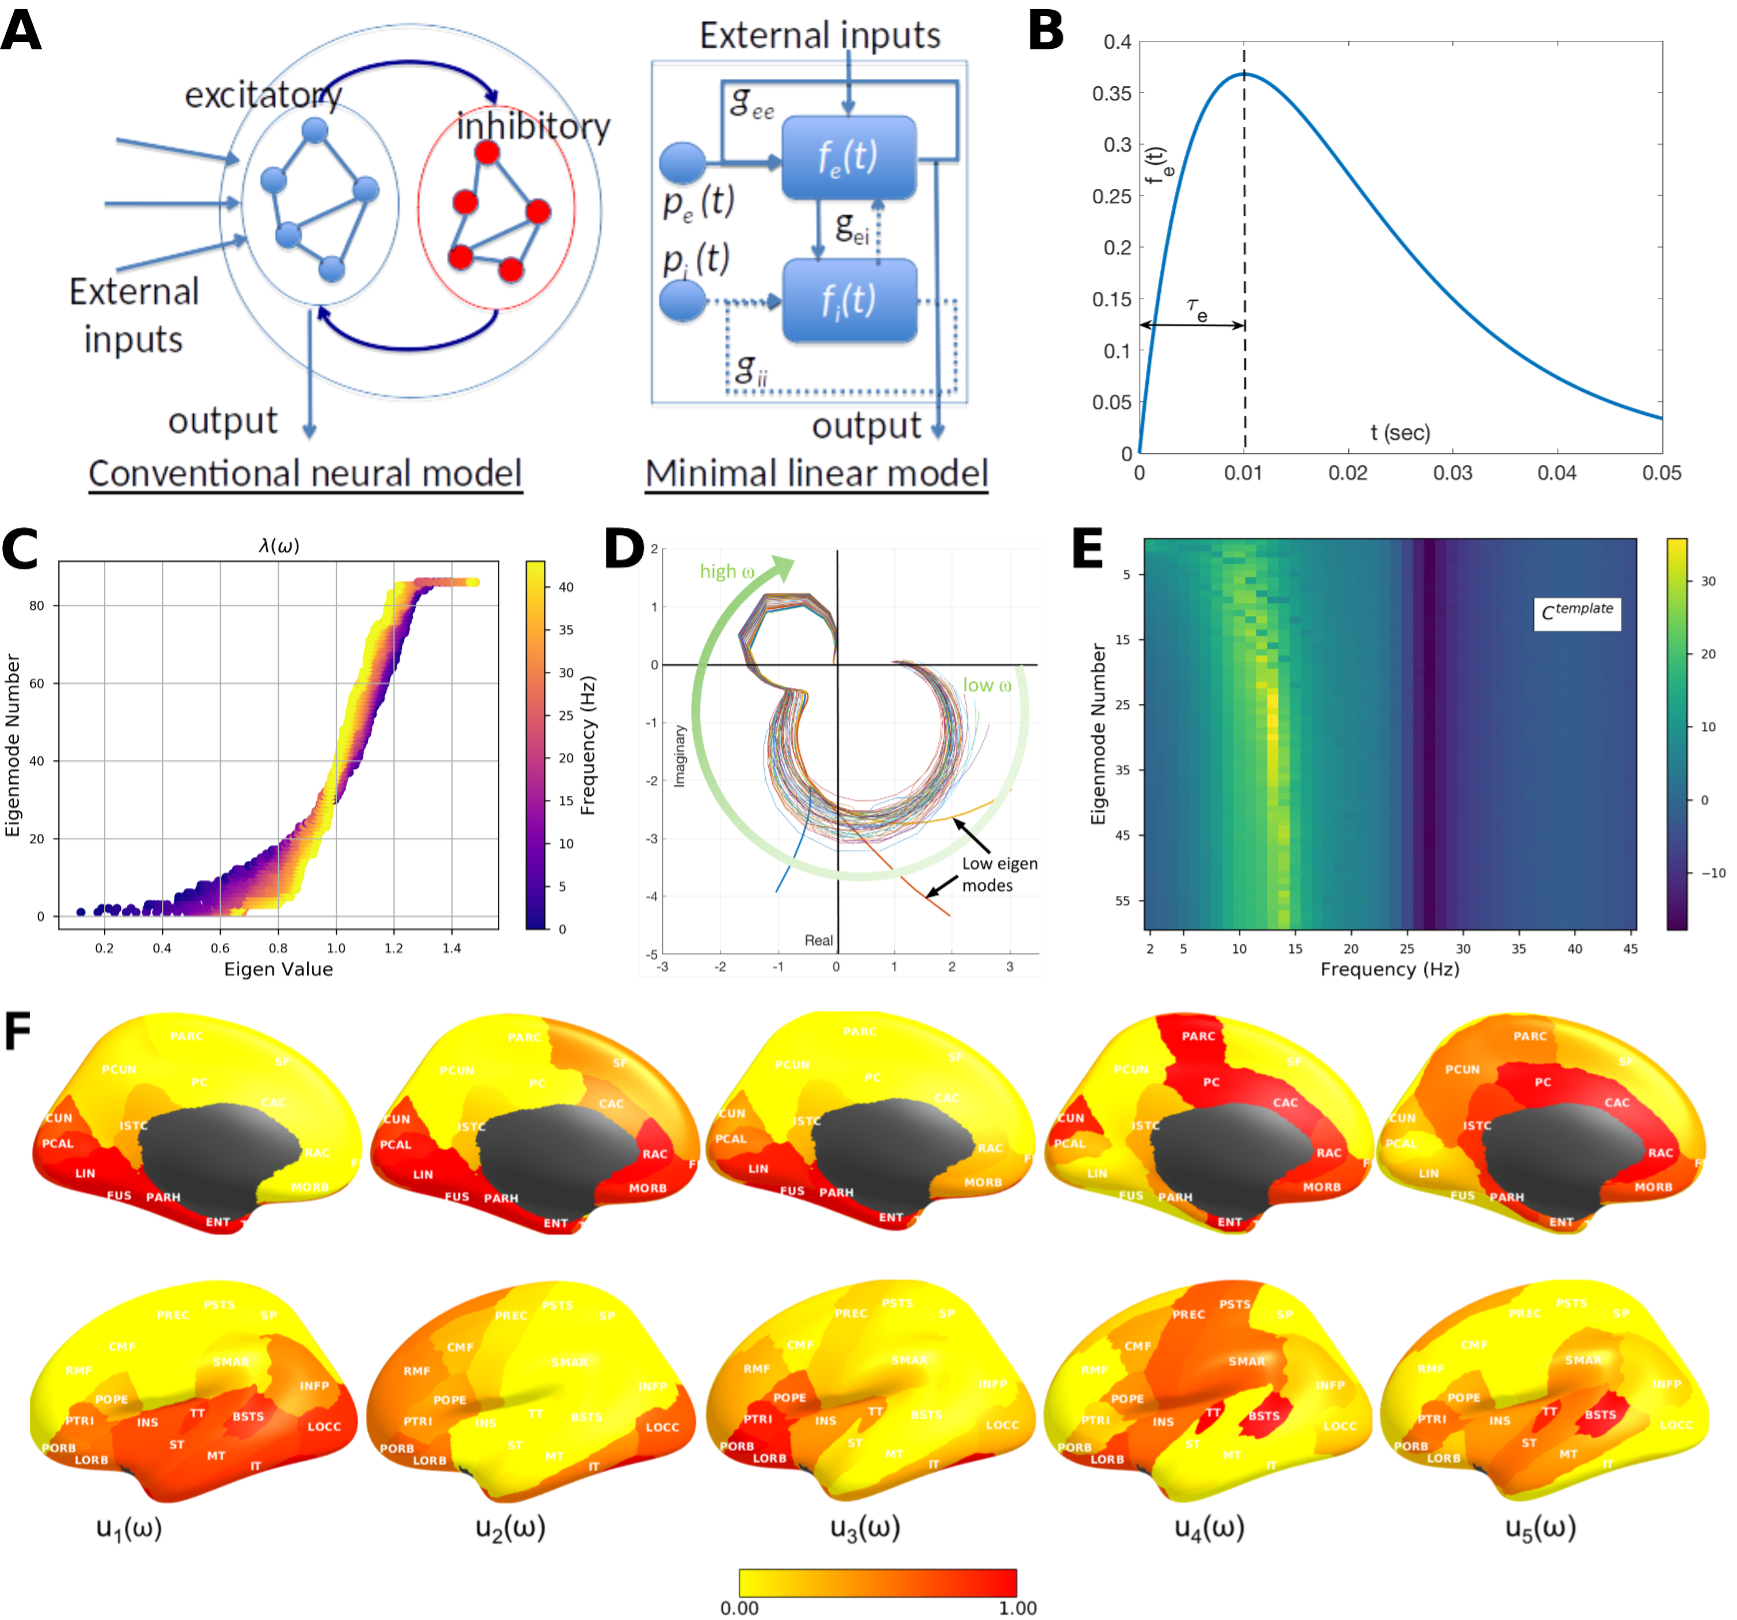
\includegraphics[scale=0.83]{../figures/chapter5/figure1.png}
    \caption{The linearized spectral graph model. (a) Conventional neural mass models instantiate a large assembly of excitatory and inhibitory neurons, which are modeled as fully connected internally. External inputs and outputs are gated through the excitatory neurons only, and inhibitory neurons are considered strictly local. The proposed linear model condenses these local assemblies into lumped linear systems $f_{e}(t)$ and $f_{i}(t)$, Gamma-shaped functions having time constants $\tau_e$ and $\tau_i$ (see panel (b)). The recurrent architecture of the two pools within a local area is captured by the gain terms $g_{ee}$, $g_{ii}$, $g_{ei}$, parameterizing the recurrents within excitatory, inhibitory and cross-populations. (c) The absolute value of eigenvalues of the complex Laplacian $\bm{\mathcal{L}}(\omega)$ are plotted against the eigenvector index. Each dot represents one eigenvalue  $\lambda(\omega)$; its color represents the frequency $\omega$ - low (blue) to high (yellow). These eigenvalues change by frequency; small eigenvalues change more compared to large ones. (d) Frequency response of each eigenmode plotted on the complex plane with default model parameters and a template structural connectome. Each curve represents the transit in the complex plane of a single eigenmode's frequency response, starting at low frequencies in the bottom right quadrant, and moving to the upper left quadrant at high frequencies. The magnitude of the response, given by the distance from the origin, suggests that most eigenmodes have two prominent lobes, roughly corresponding to lower frequency alpha rhythms and higher frequency gamma rhythms. In contrast, the lowest eigenmodes start off far from the origin, indicative of a low-pass response. (e) Magnitude of the frequency response of each eigenmode reinforces these impressions more clearly, with clear alpha peak, as well as slower rhythms. (f) The spatial patterns of the top 5 eigenmodes of $\bm{\mathcal{L}}(\omega)$, evaluated at the alpha frequency. The first 5 eigenmodes $\bm{u}_1 ... \bm{u}_5$ produce resting-state functional networks patterns; These patterns are not exclusive and greatly depend on the frequency,  model parameters, and the connectome.}
    \label{fig:sgmodel}
\end{figure}

We applied this model to and validated its construct against measured
source-reconstructed MEG recordings in healthy subjects under rest and
eyes-closed. The model closely matches empirical spatial and spectral
MEG patterns. In particular, the model displays prominent alpha and beta
peaks, and, intriguingly, the eigenmodes corresponding to the alpha
oscillations have the same posterior-dominant spatial distribution that
is repeatedly seen in eyes-closed alpha power distributions. In contrast
to existing less parsimonious models in the literature that invoke
spatially-varying parameters or local rhythm generators, to our
knowledge, this is the first account of how the spectral graph structure
of the structural connectome can parsimoniously explain the spatial
power distribution of alpha and beta frequencies over the entire brain
measurable on MEG.

\section{Methods}

\subsection{Spectral graph model development}
\textbf{Notation}. In our notation, vectors and matrices are
represented by boldface, and scalars by normal font. We denote frequency
of a signal, in Hertz, by symbol $f$, and the corresponding angular
frequency as $(\omega = 2 \pi f$. The connectivity matrix is denoted by
$\mathbf{C} = \left\{ c_{jk} \right\}$, consisting of
connectivity strength $c_{ij}$ between any two pair of regions $j,k$.

\textbf{Model summary}: Details of the Spectral Graph model (SGM) is
described in detail below. There are very few model parameters, seven in
total:
$\tau_{e}, \tau_{i}, \tau_{G}, v, g_{ii}, g_{ei}, \alpha$,
which are all global and apply at every node. See Table \ref{tab:SGM_parameters} for
their meaning, initial value and range. Note that the entire model is
based on a single equation of graph dynamics, Eq (1), which is
repeatedly applied to each level of the hierarchy. Here we used two
levels: a mesoscopic level where connectivity is all-to-all, and a
macroscopic level, where connectivity is measured from fiber
architecture. In theory, this template could be refined into finer
levels, where neural responses become increasingly non-linear, and
connectivity becomes sparser and structured.



\begin{table}
  \caption{SGM parameters values and limits}
  \label{tab:SGM_parameters}
  \centering
 \begin{tabular}{m{14em}|m{2cm}|m{2cm}|m{7em}}
 \hline
 Name & Symbol & Default Value & Optimizaiton Bounds \\
 \hline
 Excitatory Time constant & $ \tau_{e}$ & 12 ms & [5ms, 20ms] \\
 Inhibitory Time constant & $\tau_{i}$ & 3 ms & [5ms, 20ms] \\
 Graph Time constant & $\tau_{G}$ & 6 ms & [5ms, 20ms] \\
 \multicolumn{4}{l}{} \\
 Excitatory gain & $g_{ee}$ & 1 & n/a \\
 Inhibitory gain & $g_{ii}$ & 1 & [0.5, 5] \\
 Excitatory gain & $g_{ei}$ & 4 & [0.5, 5] \\
 \multicolumn{4}{l}{} \\
 Transmission velocity & $v$ & 5 m/s & [5 m/s, 20 m/s] \\
 Long-range connectivity coupling constant & $\alpha$ & 1 & [0.1, 1] \\
 \end{tabular}
\end{table}


\textbf{Canonical rate model over a graph}. We use a canonical rate
model to describe neural activity across two hierarchical levels --
local cortical mesoscopic levels and long-range macroscopic levels. At
each level of the hierarchy of brain circuits, we hypothesize a simple
linear rate model of recurrent reverberatory activity given by

\begin{equation}
\label{eq:rate_model}
\frac{dx_{e/i}(t)}{dt} = - \frac{1}{\tau_{e/i}} f_{e/i}(t) * x_{e/i}(t) + \frac{1}{\tau_{e/i}} f_{e/i}(t) * \sum_{j,k} c_{jk} x_{e/i} (t - \tau_{jk}^{v} ) + p_{e/i}(t)
\end{equation}


where $x_{e/i}(t)$ is the mean signal of the excitatory/inhibitory
populations and $p_{e/i}(t)$ is internal noise source reflecting local
cortical column computations or input. The transit of signals, from
pre-synaptic membranes, through dendritic arbors and axonal projections,
is sought to be captured into ensemble average neural impulse response
functions $f_{e}(t) = \frac{t}{\tau_{e}}\exp(-\frac{t}{\tau_{e}})$
and $f_{i}(t) = \frac{t}{\tau_{i}}\exp(-\frac{t}{\tau_{i}})$
respectively. We disregard the non-linearity of the neural response,
hence the output at the terminal to a presynaptic input $u(t)$ is the
simple convolution $x_{e}(t) = f_{e}(t)*u(t)$. The neural responses
$f_{e/i}(t)$ are Gamma-shaped responses (Figure \ref{fig:sgmodel}B)
parameterized by time constants $\tau_{e/i}$ that here represent the
end result of both synaptic membrane capacitance and the distribution of
dendritic/axonal delays introduced by the arborization. NMMs typically
use a single classical exponential decay term for membrane capacitance
only, since NMMs model highly local cell assemblies where multisynaptic
connections are infrequent and axonal and dendritic transport delays are
usually incorporated explicitly via connectivity weights and delays.
Since our lumped model was designed for relatively large cortical
regions, we employ the Gamma-shaped $f_{e/i}$ to capture not just
classical membrane capacitance but also the expected diversity of
dendritic transport delays. The dynamics of the entire assembly modeled
via a self-decaying term
$\tau_{e/i} \frac{d\mathbf{x}}{dt} \propto - f_{e/i}(t) * \mathbf{x}(t)$,
typically used in most rate or NMM models, but the difference here is
that we chose to apply convolution with neural response $f_{e/i}(t)$
within the decay process. We believe this is necessary to ensure that
the dynamics of the population cannot participate in the internal
recurrent dynamics of the region until the signal has passed through one
instance of the neuronal response. Since this neural response is meant
to capture a distribution of local circuit delays, its time constants
$\tau_{e/i}$ are purposefully far longer (up to 20ms) than expected
from membrane capacitance alone. Studies of cortical lag times using
paired electrode recordings between primary and higher cortices
demonstrate this. A short visual stimulus causes a neural response in
the ferret V1 within 20ms post-stimulus, in the primary barrel field
within 16-36ms, and the entire visual cortex becomes engaged 48-70ms
after stimulus \cite{roland_tracing_2014}. Brief deflection of a single barrel
whisker in the mouse evokes a somatotopically mapped cortical
depolarization that remains localized to its C2 barrel column only for a
few milliseconds, thence rapidly spreading to a large part of
sensorimotor cortex within tens of milliseconds, a mechanism considered
essential for the integration of sensory information
\cite{ferezou_spatiotemporal_2007, polack_long-range_2012}. Interestingly, the evoked response curve in S1
from the \textsuperscript{50} study had a prominent Gamma shape. Of
note, the duration of S1 response (\textasciitilde50ms) was considerably
longer than the time to first sensory response in C2 (7.2ms)
\cite{ferezou_spatiotemporal_2007}. Interestingly, feedback projections from higher to
lower areas take \textasciitilde50ms, hence have a much slower apparent
propagation velocity (0.15-0.25m/s) than what would be predicted by
axonal conduction alone (1-3m/s) \cite{roland_tracing_2014}.

Individual neural elements are connected to each other via connection
strengths $c_{jk}$. Let the cortico-cortical fiber conduction
speed be $v$, which here is assumed to be a global constant
independent of the pathway under question. For a given pathway
connecting regions \emph{j} and \emph{k} of length $d_{jk}$,
the conduction delay of a signal propagating from region \emph{j} to region
\emph{k} will be given by
$\tau^{v}_{jk} = \frac{d_{jk}}{v}$. Hence signals from
neighboring elements also participate in the same recurrent dynamics,
giving the second term of Eq \ref{eq:rate_model}. Equation \ref{eq:rate_model} will serve
as our canonical rate model, and will be reproduced at all levels of the
hierarchy, and only the connectivity strengths will vary depending on
the level of hierarchy we are modeling, as explained below.

\textbf{Local neural assemblies}. The local connectivities
$c_{jk}^{local}$ are assumed to be all-to-all, giving a
complete graph. Further, the axonal delays $\tau_{jk}^{v}$
associated with purely local connections were already incorporated in
the lumped impulse responses $f_{e/i}(t)$. Hence, we assert:

\begin{equation}
 c_{jk}^{local} = c_{e/i},\ \ \tau_{jk}^{v} = 0,\ \forall\ j,k\
\end{equation}

From spectral graph theory, a complete graph has all equal eigenvalues
which allows the local network to be lumped into gain constants, and the
summation removed. Indeed, rewriting $x_{e/i}(t)$ as the mean signal
of all the excitatory/inhibitory cells and setting the gains $g_{ee} = 1 - c_{e} N_{e}$ and $g_{ii} = 1 - c_{i} N_{i}$ we get

\begin{equation}
\label{eq:mean_sig}
 \frac{dx_{e/i}(t)}{dt} = -\frac{g_{ee/ii}}{\tau_{e/i}} f_{e/i}(t) * x_{e/i}(t) + p_{e/i}(t)
\end{equation}

Given the Fourier Transform pairs $\frac{d}{dt} \leftrightarrow j \omega $,
$f_{e/i}(t) \leftrightarrow F_{e/i}(\omega) = \frac{1/\tau_{e/i}^{2}}{(j \omega + 1/\tau_{e/i})^{2}}$,
we take the Fourier transform of Eq \ref{eq:rate_model} and obtain the local assembly's
frequency spectrum:

\begin{equation}
\label{eq:local_fourier}
X_{e/i}(\omega) = (j \omega + \frac{g_{ee/ii}}{\tau_{e/i}} F_{e/i}(\omega))^{-1} P_{e/i} (\omega) 
\end{equation}

Writing this in terms of transfer functions
$X_{e}(\omega) = H_{e}(\omega)P_{e}(\omega), X_{i}(\omega) = H_{i}(\omega)P_{i}(\omega)$
we get the lumped local system illustrated in Figure \ref{fig:sgmodel}.
Finally, we must also account for signals that alternate between the two
populations, which is given by the transfer function

\begin{equation}
\label{eq:transfun}
H_{ei}(\omega) = H_{e}(\omega)H_{i}(\omega) / (1 + g_{ei} H_{e}(\omega) H_{i}(\omega))
\end{equation}

We fix $g_{ee} = 1$ without loss of generality, and let the
other terms $g_{ii}, g_{ei}$ be model parameters to
be fitted. Finally, the total cortical transfer function is the sum

\begin{equation}
\label{eq:cort_transfun}
H_{local}(\omega) = H_{e}(\omega) + H_{i}(\omega) + H_{ei}(\omega)
\end{equation}

and $X_{local}(\omega) = H_{local}(\omega)P(\omega)$
represents all neural activity in this region, whether from excitatory
or inhibitory cells. The canonical local activity is therefore defined
by the Fourier transform pair: $x_{local}(t) \leftrightarrow X_{local}(\omega)$.

\subsection{Macroscopic scale: signal evolution on the entire graph}
For the macroscopic level, we use the same canonical network dynamics as
Eq \ref{eq:rate_model}, but now the inter-regional connectivity $c_{jk}$ is
non-zero and given by the structural connectome. Similarly, axonal
conductance delays are determined by fiber length and conductance speed
$\tau_{jk}^{v} = d_{jk} / v$. Further, the external
driving signals at each node is the local neural activity
$x_{local}(t)$ defined above rather than a noise process
$p(t)$. In the interest of parsimony we set each node of the
macroscopic graph to have the same internal power spectrum
$X_{local}(\omega)$ - i.e. all regions are experiencing the
same transfer function, driven by identically distributed (but of course
not identical) noise. At this scale, activity measured at graph nodes is
no longer excitatory or inhibitory, but mixed, and the corticocortical
connections are all between long, pyramidal excitatory-only cells. Thus,
for the k-th node

\begin{equation}
\label{eq:node_eq}
\frac{dx_{k}(t)}{dt} = - \frac{1}{\tau_{G}}f_{e}(t) * x_{k}(t) + \frac{\alpha}{\tau_{G}} f_{e}(t) * \sum_{j} c_{jk} x_{j}(t - \tau_{jk}^{v}) + x_{local, k}(t)
\end{equation}

Here we have introduced a global coupling constant $\alpha$, similar
to most connectivity-coupled neural mass models, that seeks to control
the relative weight given to long-range afferents compared to local
signals. We have also introduced a new time constant, $\tau_{G}$,
which is an excitatory time constant and it may be the same as the
previously used constant $\tau_{e}$. However, we allow the possibility
that the long-range projection neurons might display a different
capacitance and morphology compared to local circuits, hence we have
introduced $\tau_{G}$ (subscript $G$ is for ``graph'' or ``global'').

Stacking all equations from all nodes and using vector valued signals
$\mathbf{x}(t) = { x_{k}(t)}$, we can write

\begin{equation}
\label{eq:vec_signal}
\frac{d\mathbf{x}(t)}{dt} = - \frac{1}{\tau_{G}} f_{e}(t) * \mathbf{x}(t) + \frac{\alpha}{\tau_{G}}f_{e}(t) * C\{ \mathbf{x} ( t - \tau_{jk}^{v} )\} + \mathbf{x}_{local}(t)
\end{equation}

where the braces $\{ \cdot \}$  represent all elements of a matrix
indexed by $j,k$.

We wish to evaluate the frequency spectrum of the above. In Fourier
space, delays become phases; hence we use the transform pairs
$\frac{d\mathbf{x}}{dt} \leftrightarrow j \omega \mathbf{X}(\omega)$ and
$\mathbf{x}(t - \tau) \leftrightarrow e^{- j\tau\omega}\mathbf{X}(\omega)$.
Therefore, define a "complex connectivity matrix" at any given angular
frequency $\omega$ as
$\mathbf{C}^{\mathbf{*}}(\omega) ={ c_{jk} \exp ( - j \omega \tau^{v}_{jk} ) }$.
We then define a normalized complex connectivity matrix at frequency
$\omega$ as

\begin{equation}
\label{eq:comp_conn}
\mathcal{C}(\omega) = \textrm{diag}(\frac{1}{\mathbf{\deg}}) \mathbf{C}^{\mathbf{*}}(\omega)
\end{equation}

where the degree vector $\mathbf{\deg}$ is defined as
$\deg_{k}= \sum_{j} c_{jk}$. Taking the Fourier transform
of Equation \ref{eq:vec_signal}, we get

\begin{equation}
\label{eq:fourier_sig}
(j \omega \mathbf{X}(\omega) + \frac{1}{\tau_{G}} F_{e}(\omega) (\mathbf{I} - \alpha \mathcal{C}(\omega)) \mathbf{X}(\omega)) = H_{local}(\omega) \mathbf{P}(\omega) 
\end{equation}

where we assumed identically distributed noise signals driving both the
excitatory and inhibitory local populations at each node, such that
$P_{e,k}(\omega) = P_{i,k}(\omega) = P_{k}(\omega)$ at the $k$-th node.
We then collected all nodes' driving inputs in the vector
$\mathbf{P}(\omega) = { P_{k}(\omega), \forall k }$.
Here, we define the complex Laplacian matrix

\begin{equation}
\label{eq:clap}
\mathcal{L}(\omega) = \mathbf{I} - \alpha \mathcal{C}(\omega)
\end{equation}

where $\mathbf{I}$ is the identity matrix of size $N \times N$. This
complex Laplacian will be evaluated via the eigen-decomposition

\begin{equation}
\label{eq:decomp}
\mathcal{L}(\omega) = \mathbf{U}(\omega)\mathbf{\Lambda}(\omega)\mathbf{U}(\omega)^{H}
\end{equation}

where
$\mathbf{\Lambda}(\omega) = \textrm{diag}([\lambda_{1}(\omega),\ldots,\lambda_{N}(\omega)])$
is a diagonal matrix consisting of the eigenvalues of the complex
Laplacian matrix of the connectivity graph $\mathcal{C}(\omega)$, at
the angular frequency $\omega$.

Hence
\begin{equation}
\label{eq:lap_sgm}
\mathbf{X}(\omega) = (j\omega\mathbf{I} + \frac{1}{\tau_{G}} F_{e}(\omega) \mathcal{L}(\omega))^{-1} H_{local}(\omega)\mathbf{P}(\omega)
\end{equation}

where we invoke the eigen-decomposition of $\mathcal{L}(\omega)$, and
that $\mathbf{U}(\omega){\mathbf{U}(\omega)}^{H} = \mathbf{I}$. It
can then be shown easily that

\begin{equation}
\label{sgm}
\mathbf{X}(\omega) =\sum_{i}\frac{\mathbf{u}_{i}(\omega)\mathbf{u}_{i}^{H}(\omega)}{j\omega + \frac{1}{\tau_{G}}\lambda_{i}(\omega) F_{e}(\omega)} H_{local}(\omega) \mathbf{P}(\omega)
\end{equation}

This is the steady state frequency response of the whole brain dynamics.
In steady state, we assume that each cortical region is driven by
internal noise that spans all frequencies, i.e. white noise. Hence, we
assume that the driving function $\mathbf{p}(t)$ is an uncorrelared
Gaussian noise process, such that
$\mathbf{P}(\omega) = \mathbb{I}$ where $\mathbb{l}$ is a vector of
ones. This asserts identical cortical responses at each brain region.

\subsection{Experimental Procedures}
\textbf{Study cohort}. We acquired MEG, anatomical MRI, and diffusion
MRI for 36 healthy adult subjects (23 males, 13 females; 26 left-handed,
10 right-handed; mean age 21.75 years (range: 7-51 years). All study
procedures were approved by the institutional review board at the
University of California at San Francisco (UCSF) and are in accordance
with the ethics standards of the Helsinki Declaration of 1975 as revised
in 2008.

\textbf{MRI.} A 3 Tesla TIM Trio MR scanner (Siemens, Erlangen,
Germany) was used to perform MRI using a 32-channel phased-array
radiofrequency head coil. High-resolution MRI of each subject's brain
was collected using an axial 3D magnetization prepared rapid-acquisition
gradient-echo (MPRAGE) T1-weighted sequence (echo time {[}TE{]} = 1.64
ms, repetition time {[}TR{]} = 2530 ms, TI = 1200 ms, flip angle of 7
degrees) with a 256-mm field of view (FOV), and 160 1.0-mm contiguous
partitions at a 256×256 matrix. Whole-brain diffusion weighted images
were collected at b = 1000$s/mm^{2}$ with 30 directions using 2-mm
voxel resolution in-plane and through-plane.

\textbf{Magneto-encephalography (MEG) data}. MEG recordings were
acquired at UCSF using a 275-channel CTF Omega 2000 whole-head MEG
system from VSM MedTech (Coquitlam, BC, Canada). All subjects were
instructed to keep their eyes closed for five minutes while their MEGs
were recorded at a sampling frequency of 1200 Hz.

\subsection{Data Processing}

\textbf{Region Parcellations}. The T1-weighted images were parcellated
into 68 cortical regions and 18 subcortical regions using the using the
Desikan-Killiany atlas available in the FreeSurfer software
\cite{Fischl2002}. To do this, the subject specific T1-weighted
images were back-projected to the atlas using affine registration, as
described in our previous studies \cite{abdelnour_network_2014,owen_structural_2013}.

\textbf{Structural Connectivity Networks.} We constructed different
structural connectivity networks with the same Desikan-Killiany
parcellations to access the capabilities of our proposed model. Firstly,
we obtained openly available diffusion MRI data from the MGH-USC Human
Connectome Project to create an average template connectome. As in our
previous studies \cite{abdelnour_network_2014,owen_structural_2013}, subject specific structural
connectivity was computed on diffusion MRI data: \emph{Bedpostx} was
used to determine the orientation of brain fibers in conjunction with
\emph{FLIRT}, as implemented in the \emph{FSL} software
\cite{Jenkinson2012}. In order to determine the elements of the
adjacency matrix, we performed tractography using \emph{probtrackx2}. We
initiated 4000 streamlines from each seed voxel corresponding to a
cortical or subcortical gray matter structure and tracked how many of
these streamlines reached a target gray matter structure. The weighted
connection between the two structures $c_{i,j}$, was defined as the
number of streamlines initiated by voxels in region $\i$that
reach any voxel within region $j$, normalized by the sum of the source
and target region volumes
($c_{i,j} = \frac{\textrm{streamlines}}{v_{i} + v_{j}}$). This
normalization prevents large brain regions from having high connectivity
simply due to having initiated or received many streamlines. Afterwards,
connection strengths are averaged between both directions ($c_{i,j}$
and $c_{j,i}$) to form undirected edges. It is common in neuroimaging
literature to threshold connectivity to remove weakly connected edges,
as this can greatly influence the implied topology of the graph. In our
work, we chose not to apply further thresholding, as unlike conventional
graph theoretic metrics, linear models of spread and consequently
network eigenmodes are relatively insensitive to implied topology
induced by presence (or lack) of weak nonzero connections. However, to
determine the geographic location of an edge, the top 95\% of non-zero
voxels by streamline count were computed for both edge directions. The
consensus edge was defined as the union between both post-threshold
sets.

\textbf{MEG processing and source reconstruction.} MEG recordings were
down-sampled from 1200 Hz to 600 Hz, then digitally filtered to remove
DC offset and any other noisy artifact outside of the 1 to 160 Hz
bandpass range. Since MEG data are in sensor space, meaning they
represent the signal observable from sensors placed outside the head,
this data needs to be ``inverted'' in order to infer the neuronal
activity that has generated the observed signal by solving the so-called
inverse problem. Several effective methods exist for performing
\emph{source localization} \cite{wipf_robust_2010,zumer_probabilistic_2008,jerbi_localization_2004}. Here we eschew the
common technique of solving for a small number of discrete dipole
sources which is not fully appropriate in the context of inferring
resting state activity, since the latter is neither spatially sparse not
localized. Instead, we used adaptive spatial filtering algorithms from
the NUTMEG software tool written in house \cite{dalal_nutmeg_2004} in MATLAB
(The MathWorks, Inc., Natick, Massachusetts, United States). To prepare
for source localization, all MEG sensor locations were co-registered to
each subject's anatomical MRI scans. The lead field (forward model) for
each subject was calculated in NUTMEG using a multiple local-spheres
head model (three-orientation lead field) and an 8 mm voxel grid which
generated more than 5000 dipole sources, all sources were normalized to
have a norm of 1. Finally, the MEG recordings were projected into source
space using a beamformer spatial filter. Source estimates tend to have a
bias towards superficial currents and the estimates are more error-prone
when we approach subcortical regions, therefore, only the sources
belonging to the 68 cortical regions were selected to be averaged around
the centroid. Specifically, all dipole sources were labeled based on the
Desikan-Killiany parcellations, then sources within a 20 mm radial
distance to the centroid of each brain region were extracted, the
average time course of each region's extracted sources served as
empirical resting-state data for our proposed model.

\textbf{Alternative benchmark model for comparison.} In order to put the
proposed model in context, we also implemented for comparison a
Wilson-Cowan neural mass model \cite{destexhe_wilson-cowan_2009,wilson_mathematical_1973,muldoon_stimulation-based_2016} (add criticism citation here) with
similar dimensionality. Although NMMs like this can and have been
implemented with regionally varying local parameters, here we enforced
uniform, regionally non-varying local parameters, meaning all
parcellated brain regions shared the same local and global parameters.
This is a fair comparison since the proposed model is also regionally
non-varying. The purpose of this exercise is to ascertain whether a
non-regional NMM can also predict spatial power variations purely as a
consequence of network transmission, like the proposed model, using the
same model optimization procedure (see below). This NMM incorporates a
transmission velocity parameter that introduces a delay based on fiber
tract lengths extracted from diffusion MRI, but, unlike our model, does
not seek to explicitly evaluate a frequency response based on these
delays.

\subsection{Model Optimization}
We computed \emph{maximum a posteriori} estimates for parameters under a
flat non-informative prior. A simulated annealing optimization algorithm
was used for estimation and provided a set of optimized parameters
$\{\tau_{e}, \tau_{i}, \tau_{c}, g_{ei}, g_{ii}, \alpha, \upsilon\}$.
We defined a data likelihood or goodness of fit (GOF) as the Pearson
correlation between empirical source localized MEG power spectra and
simulated model power spectra, averaged over all 68 regions of a
subject's brain. The proposed model has only seven global parameters as
compared to neural mass models with hundreds of parameters, and is
available in closed-form. To improve the odds that we capture the global
minimum, we chose to implement a probabilistic approach of simulated
annealing \cite{Kirkpatrick1983}. The algorithm samples a set of
parameters within a set of boundaries by generating an initial trial
solution and choosing the next solution from the current point by a
probability distribution with a scale depending on the current
``temperature'' parameter. While the algorithm always accepts new trial
points that map to cost-function values lower than the previous
cost-function evaluations, it will also accept solutions that have
cost-function evaluations greater than the previous one to move out of
local minima. The acceptance probability function is
$1/(1 + \frac{\mathrm{\Delta}}{e^{\max(T)}})$, where T is the current
temperature and ∆ is the difference of the new minus old cost-function
evaluations. The initial parameter values and boundary constraints for
each parameter are given in Supplementary Table 1. All simulated
annealing runs were allowed to iterate over the parameter space for a
maximum of $N_{p} \times 3000$ iterations, where $N_{p}$ is the
number of parameters in the model. As a comparison, we performed the
same optimization procedure to a regionally non-varying Wilson-Cowan
neural mass model \cite{wilson_mawilson_mathematical_1973,muldoon_stimulation-based_2016}.

\section{Results}
\subsection{Graph Laplacian eigenmodes mediate a diversity of frequency
responses}

First, we demonstrate the spectra produced by graph eigenmodes as per
our theory using default choices of model parameters. Figure \ref{fig:sgmodel}C
shows the eigen-spectrum of the complex Laplacian, with eigenvalue
magnitude ranging from 0 to 1. The absolute value of eigenvalues of the
complex Laplacian $\mathcal{L}(\omega)$ are plotted against the
eigenvector index. Each dot represents one eigenvalue
$\lambda(\omega)$; its color represents the frequency $\omega$ - low
(blue) to high (yellow). Clearly, these eigenvalues change somewhat by
frequency. Small eigenvalues undergo a larger shift due to frequency,
while the large ones stay more stable and tightly clustered around the
nominal eigenvalue (i.e. at $\omega = 0$). Each eigenmode produces a
frequency response based on its frequency-dependent eigenvalue
(Figure \ref{fig:sgmodel}D, E}). Figure \ref{fig:sgmodel}D shows the transit in the
complex plane of a single eigenmode's frequency response, starting at
low frequencies in the bottom right quadrant, and moving to the upper
left quadrant at high frequencies. The magnitude, given by distance from
origin, suggests that most eigenmodes have two prominent lobes, one
roughly corresponding to lower frequency alpha rhythm and another
corresponding to higher frequency beta or gamma rhythms, respectively.
In contrast, the lowest few eigenmodes start off far from the origin,
indicative of a low-pass response. The magnitude of these complex-valued
curves shown in figure 1E reinforces these impressions, with clear alpha
peak, as well as slower rhythms of the lowest eigenmodes. The spectral
profile of the eigenmodes, especially the peak frequencies, are
sensitive to the choice of model parameters as demonstrated below.

The spatial patterns of the first 5 eigenmodes of
$\mathcal{L}(\omega)$, evaluated at the alpha peak of 10 Hz, are shown
in Figure \ref{fig:sgmodel}F. Eigenmodes
$\mathbf{u}_{\mathbf{1 - 4}}$ produce posterior and temporal spatial
patterns, including many elements of the \textbf{default mode network;}
\(\mathbf{u}_{\mathbf{4}}\) resembles the \textbf{sensorimotor network};
and \(\mathbf{u}_{5}\) the \textbf{structural core} of the human
connectome. However, these patterns are not exclusive and greatly depend
on the frequency at which they are evaluated, as well as the model
parameters. Higher eigenmodes are especially sensitive to axonal
velocity and frequency (not shown here).
